%% Chapter 6: Results
\chapter{Results}
\label{chapter:results}

\graphicspath{ {report/C6 Results/assets/} } 

% ** remember to include results of all early, prelim experiments including the OpenBCI experiments and periodogram plots of the alpha energy experiments with the initial Frankenstein hardware.

\section{Hardware Verification and Testing}
This section details the results of the various verification tests mentioned in Section \ref{subsection:testing-verification-method-c4}. The purpose of these tests was to verify that all core components of the designed system performed as expected. After basic tests to verify firmware integrity and communication with the ESP32-based target board passed, the digital signal processing (DSP) system was investigated. The results of important diagnostic tests are detailed below. Throughout this section, "the hardware" refers to the electronic hardware introduced in Section \ref{subsection:electronic-hardware-proto} and pictured in Figure \ref{fig:esp-hardware}.

\subsection{DSP system}
As explained in Section \ref{fig:digital-system-c5}, the DSP system is crucial for preparing analogue signals acquired from hardware prior to decoding. In order to test several components of this system simultaneously, a square wave signal $x[n]$ at fundamental frequency $f_x^{(0)}=12$Hz was fed to the ADC of the ESP32. Sampling was set to $f_s=256$Hz and where applicable, downsampling to $f_s^'=64$Hz was used. Owing to the lack of access to a signal generator or other laboratory equipment, the input signal $x[n]$ was generated using a hardware timer on board the ESP32. This experiment was designed to test the following components of the DSP system as follows:
\begin{enumerate}
    \item \textbf{sampling}: a basic sanity check to verify that a square wave at 12Hz was indeed measured by the ADC. This also offered a means of inspecting the consistency (both in amplitude and frequency) of the measured signal.
    \item \textbf{filtering}: the input signal $x[n]$ was filtered by the onboard digital low-pass filter described in Section \ref{subsection:digital-filtering} to yield $y[n]$. Given the filter's corner frequency of $f_c=26$Hz, $y[n]$ should only contain the fundamental frequency $f_x^{(0)}=12$Hz since higher order harmonics of the square wave input at $\{f_x^{(k)} |f_x^{(k)}=(2k-1)f_x^{(0)}, \, k=2,3, \dots\} = \{36\text{Hz}, 60\text{Hz}, \dots\}$ should be fully attenuated. Furthermore, the measured spectrum of $y[n]$ offers a way to compare the actual and designed behaviour of the filter.
    \item \textbf{downsampling}: a simple check to confirm that, given all prior design decisions, downsampling does not distort the originally measured signal excessively in the frequency band of interest (around $7-12$Hz). With low-pass filtering in place, there should be no aliasing or artefacts introduced.
\end{enumerate}

All results reported below were computed on the hardware itself, i.e.: all DSP operations (sampling, filtering, resampling) were computed on-device as would happen in a real application. Figures were then plotted using \texttt{Matplotlib}, an open source Python library.

\subsubsection{Sampling}
Figure \ref{fig:sq-wave-time-c6} shows the filtered signal $y[n]$ against the measured input square wave $x[n]$. From visual inspection, $x[n]$ appears to have very consistent frequency and amplitude as desired. $y[n]$ shows marginal phase lag and slight inconsistencies in amplitude compared to the ideal output $y^*[n] = \frac{4}{\pi}\sin(2\pi f_x^{(0)}n)$. However, these slight deviations are certainly tolerable and would make little to no difference to the success of subsequent decoding algorithms.

\begin{figure}[h]
    \centering
    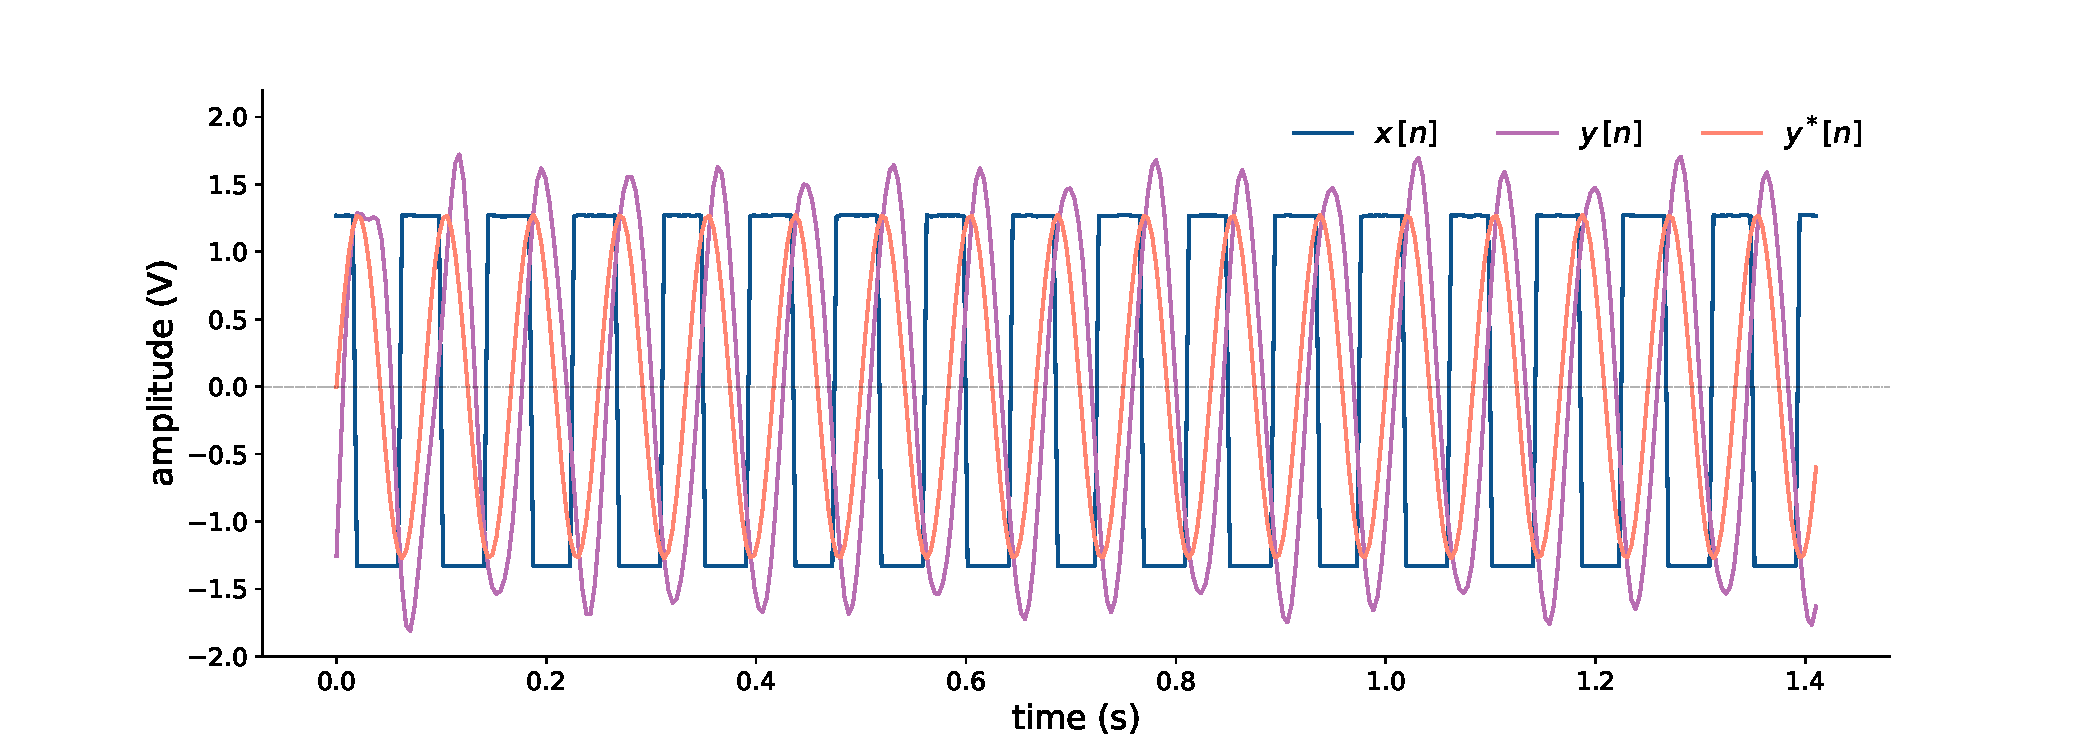
\includegraphics[width=\textwidth]{sq_wave_filtering_time}
    \caption[Time domain plot showing the measured square wave signal together with the digitally-filtered output signal.]{Time domain plot showing the measured square wave signal $x[n]$ together with the digitally-filtered output signal $y[n]$ designed to retain only the fundamental frequency $f_x^{(0)}$ of $x[n]$. The ideal output signal $y^*[n]$ represents a sinsuoid at frequency $f_x^{(0)}$: $y^*[n] = \frac{4}{\pi}\sin(2\pi f_x^{(0)}n)$.}
    \label{fig:sq-wave-time-c6}
\end{figure}

\subsubsection{Filtering}
Figure \ref{fig:sq-wave-spectra-c6} shows PSD estimates $\hat{P}_x(\omega)$ and $\hat{P}_y(\omega)$ of $x[n]$ and $y[n]$ respectively in the form of periodograms. Confirming the time domain representation in Figure \ref{fig:sq-wave-time-c6}, $\hat{P}_x(\omega)$ shows power peaks at the odd numbered harmonics of $x[n]$. This can be explained by the Fourier series expansion of an ideal square wave at fundamental frequency $f^{(0)}$ with 50\% duty cycle:
\begin{equation}
    x[n]=\frac{4}{\pi} \sum_{k=1}^{\infty} \frac{\sin (2 \pi(2 k-1) f^{(0)} n)}{2 k-1},
    \label{eq:fourier-series-sinsusoid}
\end{equation}
which is nothing but an infinite sum of sinusoids whose amplitudes decay with frequency. Notice that only odd-numbered harmonics in (\ref{eq:fourier-series-sinsusoid}) are non-zero. Therefore, the ideal spectrum $P_x(\omega)$ of $x[n]$ should be an impulse train at frequencies $(2k-1)f_x^{(0)}, \, k\geq2, \, k\in\mathbb{Z}$. 

While not quite impulses, power peaks of $\hat{P}_x(\omega)$ in Figure \ref{fig:sq-wave-spectra-c6} are clearly visible at the odd-numbered harmonics at 26Hz, 60Hz and so on. The spectrum of the filtered signal, $\hat{P}_y(\omega)$, shows very little distortion in the pass-band between 0 and $f_c=26$Hz, as well as impressively steep roll-off for $f>f_c$. As a result, only the fundamental frequency of $x[n]$ is captured in $y[n]$, as desired. Attenuation of higher frequency harmonics in $x[n]$ by the digital filter is evidently very effective and meets the design criteria stated in Section \ref{subsection:digital-filtering}: stop-band attenuation is approximately 80dB, as can be seen in the power difference between $\hat{P}_x(\omega)$ and $\hat{P}_y(\omega)$ at 60Hz, for example.

\begin{figure}[!htb]
    \centering
    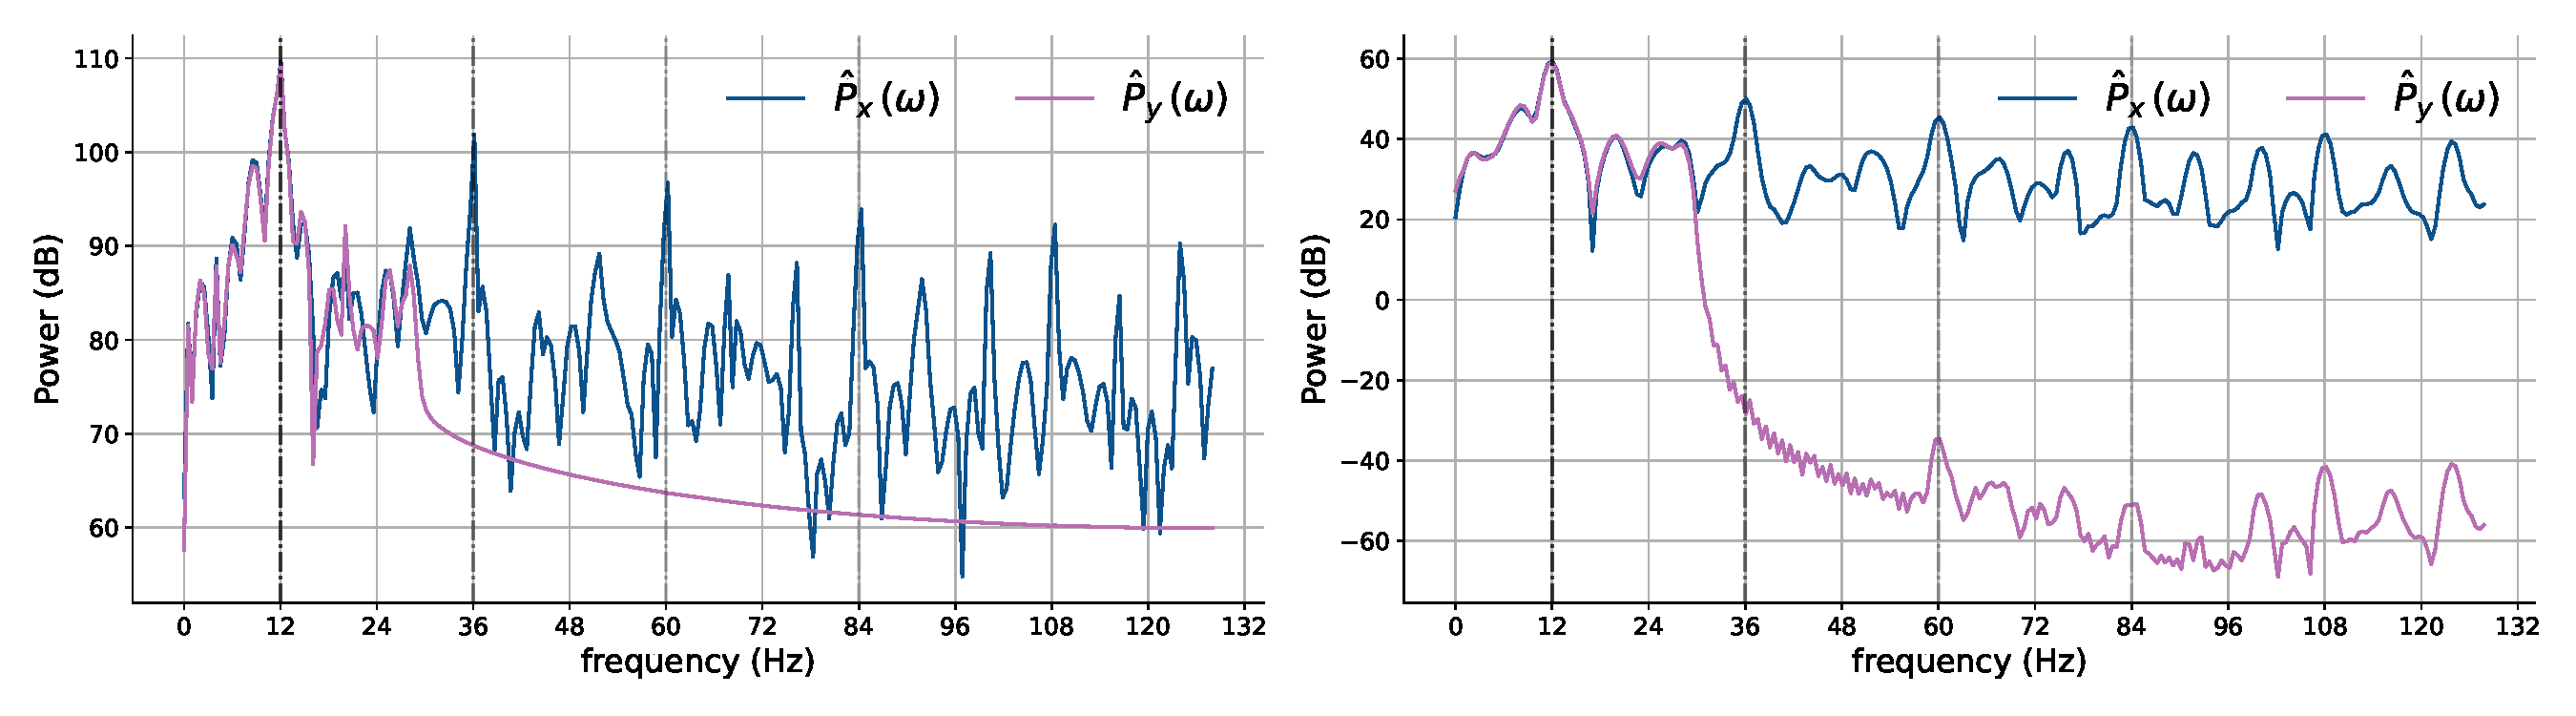
\includegraphics[width=\textwidth]{sq_wave_filtering_spectra}
    \caption[PSD estimates of a measured input signal and its filtered output]{Standard periodogram (left) and Welch-averaged periodogram (right) representing PSD estimates of measured input signal $x[n]$ and filtered output $y[n]$. Dashed vertical lines mark $f_x^{(0)}$ and odd-numbered harmonics of $x[n]$.}
    \label{fig:sq-wave-spectra-c6}
\end{figure}

\subsubsection{Downsampling}

\begin{figure}[h]
    \centering
    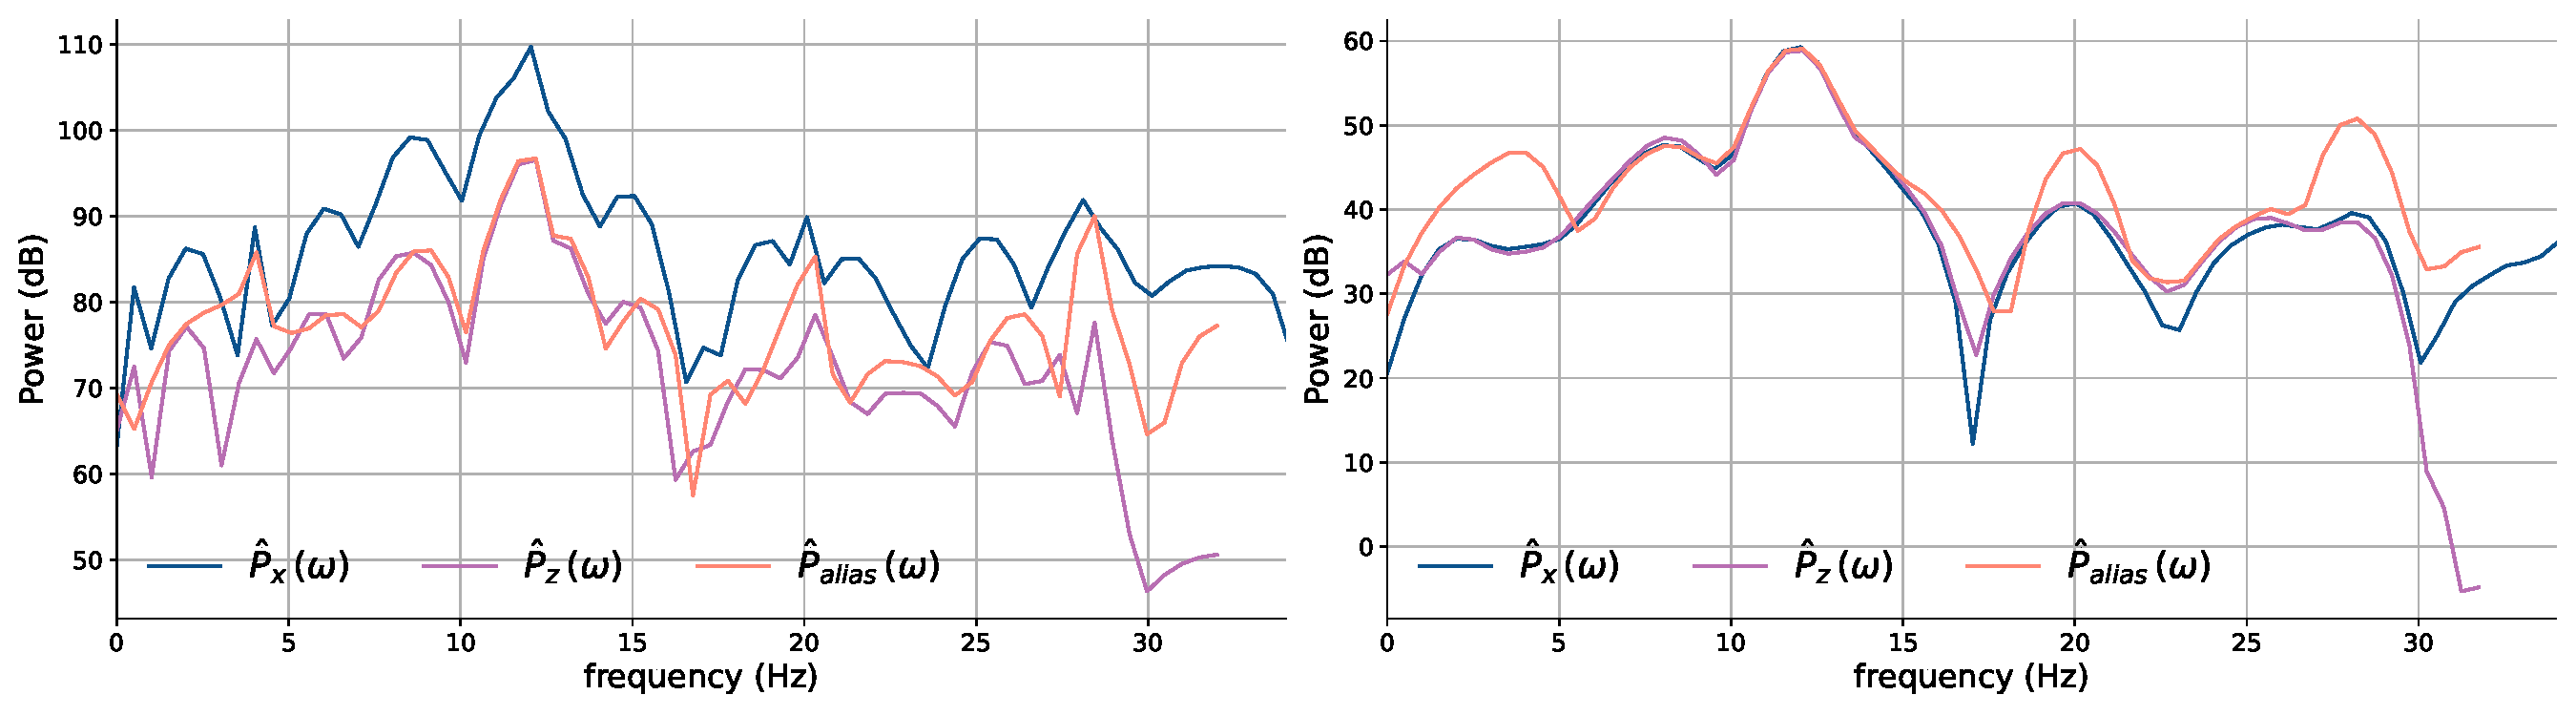
\includegraphics[width=\textwidth]{sq_wave_filtering_ds_spectra}
    \caption[PSD estimates of an input signal, filtered and downsampled version and a downsampled version without filtering.]{Standard periodogram (left) and Welch-averaged periodogram (right) representing PSD estimates $\hat{P}_x(\omega)$ and $\hat{P}_z(\omega)$ of input $x[n]$ and filtered, downsampled output $z[n]$ respectively. $\hat{P}_{\text{alias}}(\omega)$ shows the estimated spectrum of a downsampled version of $x[n]$ \textit{without} prior low-pass filtering}.
    \label{fig:sq-wave-ds-spectra-c6}
\end{figure}

\subsection{Hardware and data acquisition}

\begin{figure}[htp]
\subfloat[eyes open]{%
  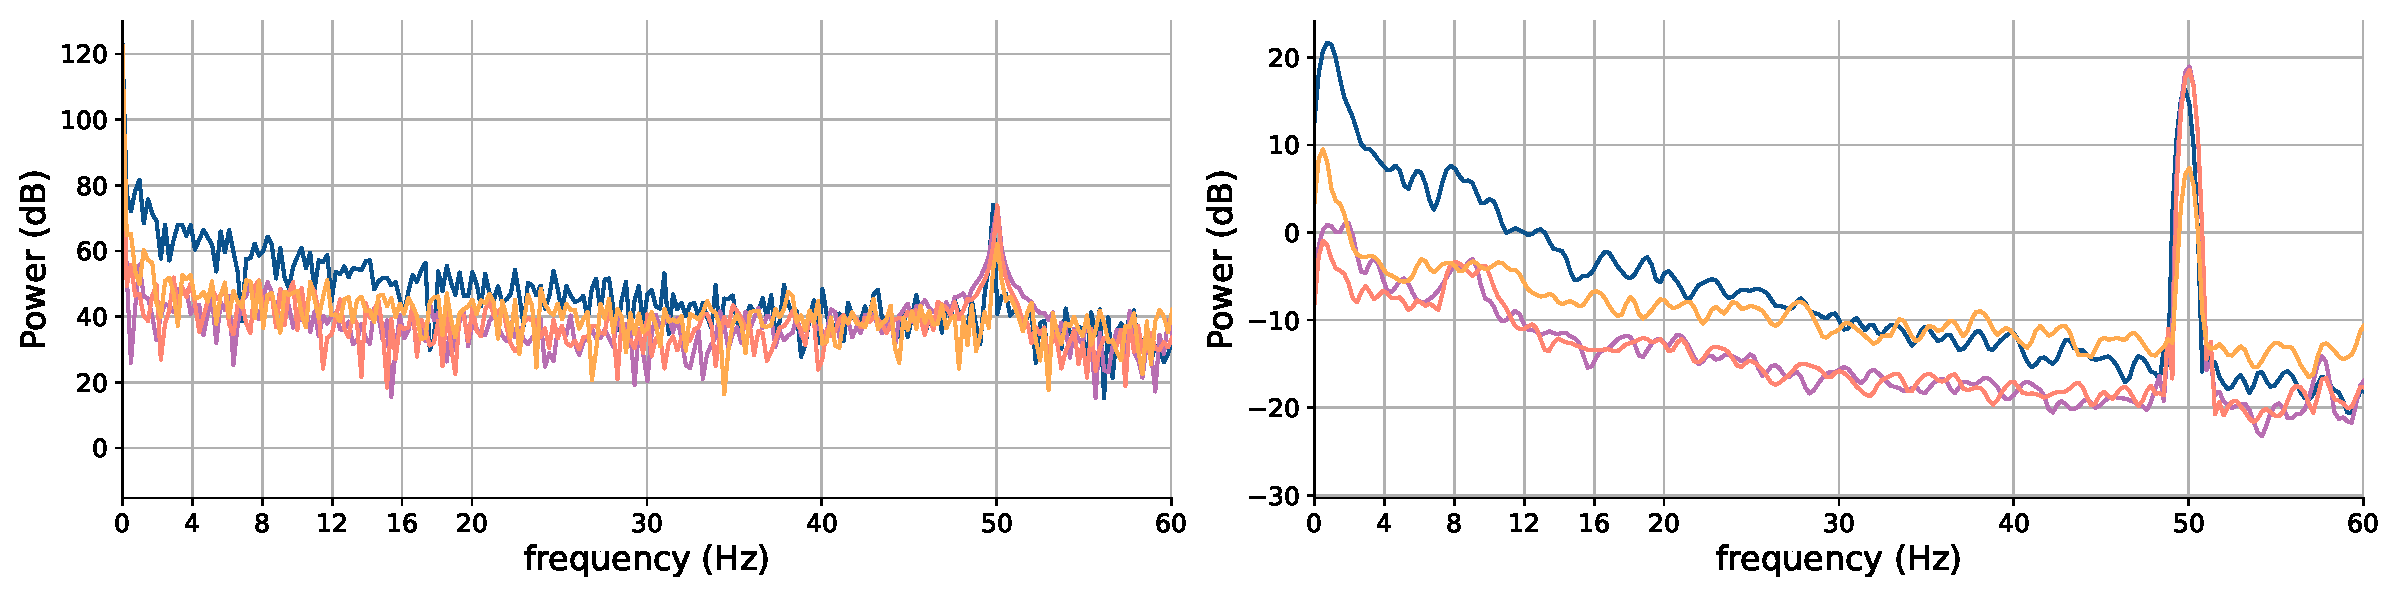
\includegraphics[clip,width=\columnwidth]{eyes_open_alpha_spectra_N1024.pdf}%
}

\subfloat[eyes closed]{%
  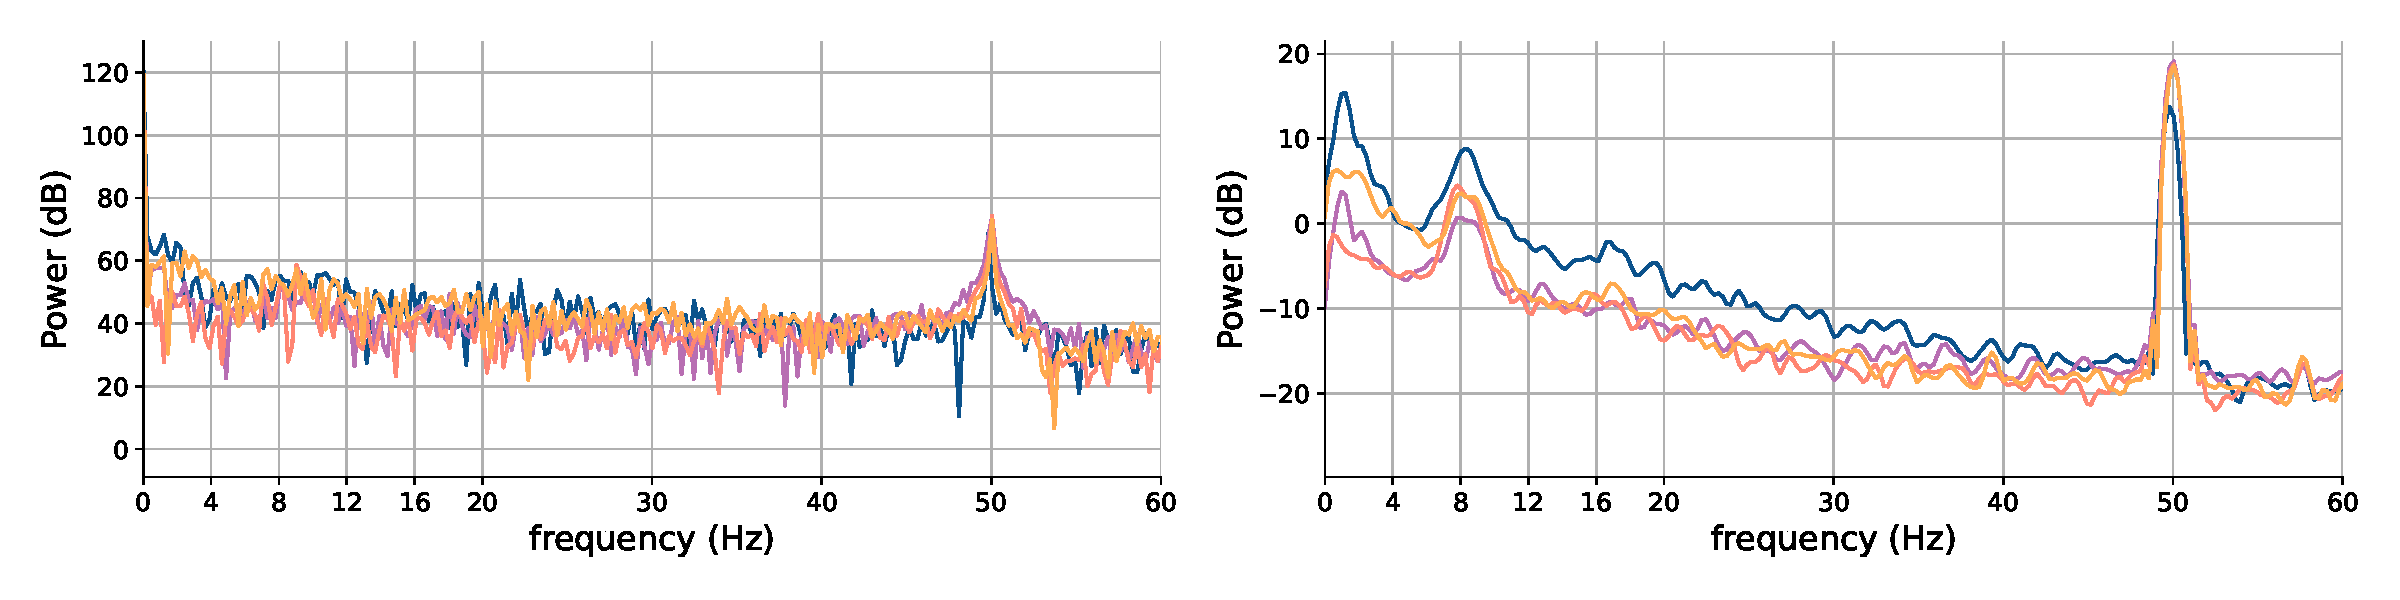
\includegraphics[clip,width=\columnwidth]{eyes_closed_alpha_spectra_N1024.pdf}%
}
\caption[Alpha band test: periodograms showing $N=1024$ point PSD estimates for EEG signals measured from a subject in two distinct states: with eyes open and eyes closed.]{\textbf{Alpha band test}: periodograms showing $N=1024$ point PSD estimates for EEG signals measured from a subject in two distinct states: with eyes open and eyes closed. Data was acquired using the early hardware prototype in Figure \ref{fig:frakenstein-hardware}. Attention should be given to signal power around $8-10$Hz (alpha band). In both (a) and (b), the left subplot shows a standard, non-windowed periodogram accompanied by a Welch-averaged periodogram to the right. Different coloured traces represent independent trials.}
\end{figure}


\section{Experimental Decoding Results}

%% Experiments with varying Nt: GCCA
\begin{figure}[htp]
\subfloat[$T = 0.75$s ($N_s=192, N_s'=48$)]{%
    \label{subfig:gcca-nt-ns48}
    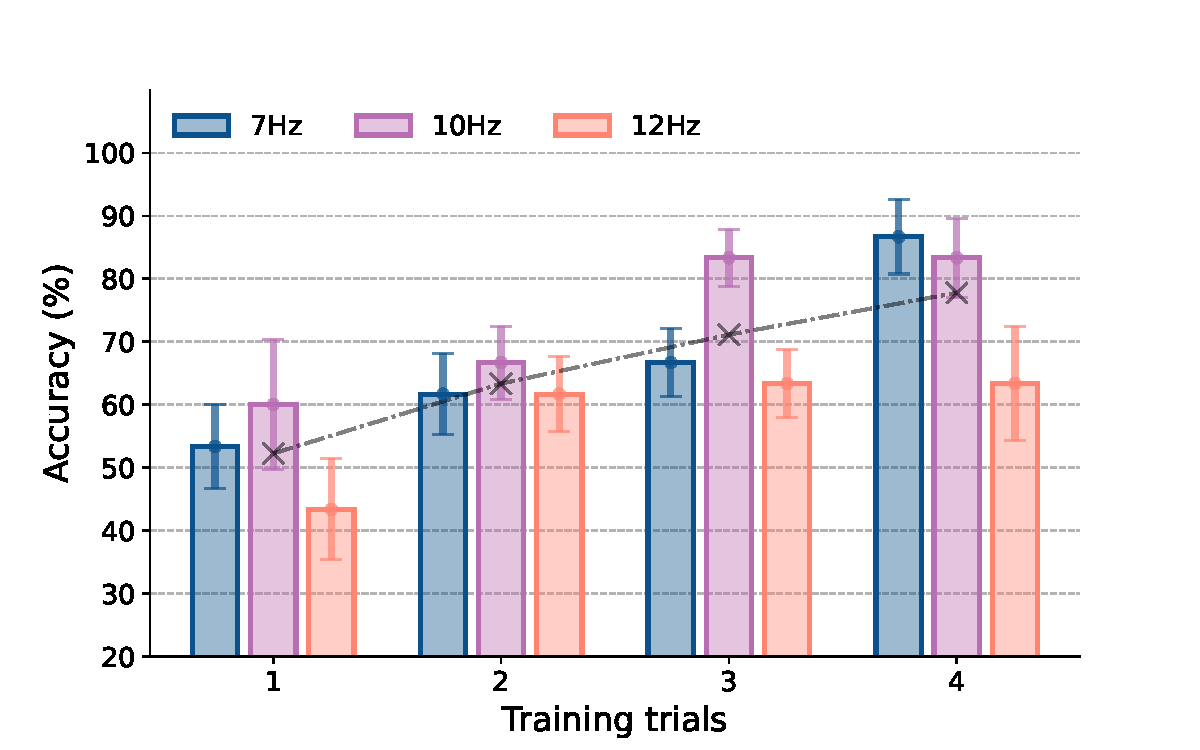
\includegraphics[clip,width=0.49\columnwidth]{report/C6 Results/assets/acc_Nt_gcca_Ns48.pdf}%
    \label{subfig:gcca-nt-ns64}
}
\hfill
\subfloat[$T = 1$s ($N_s=256, N_s'=64$)]{%
    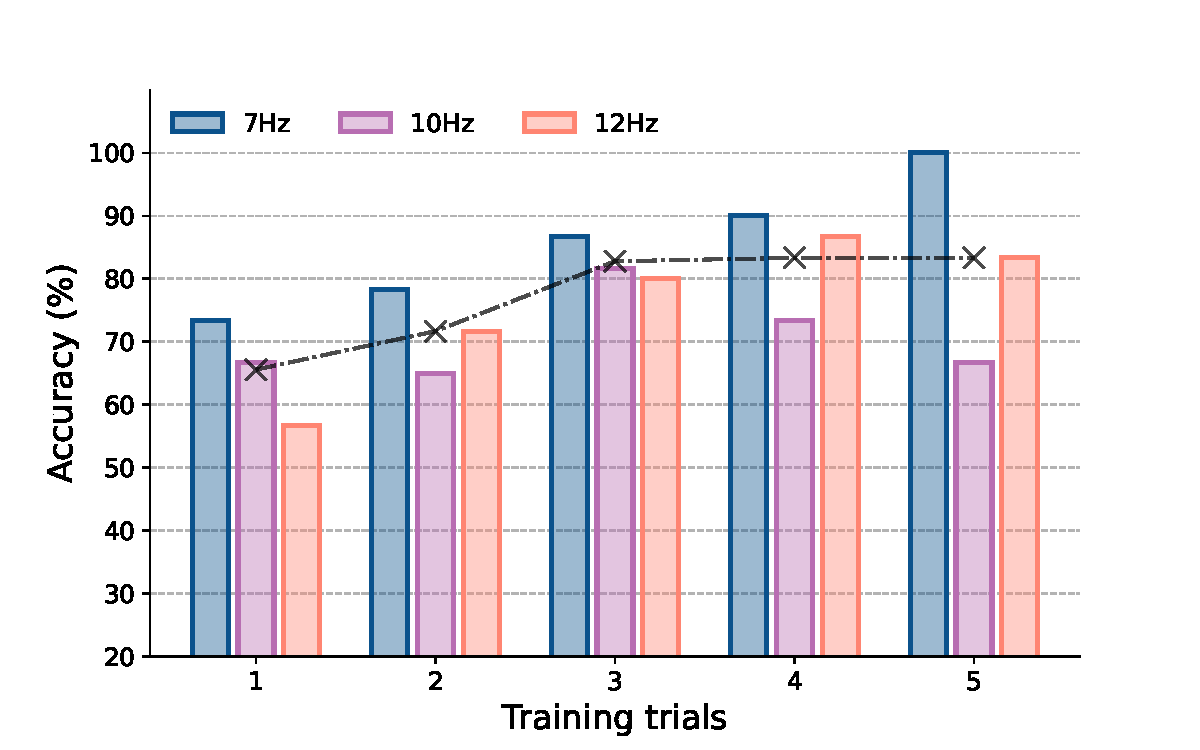
\includegraphics[clip,width=0.49\columnwidth]{report/C6 Results/assets/acc_Nt_gcca_Ns64.pdf}%
    \label{subfig:gcca-nt-ns64}
}
% ensure there is a space below here!

\subfloat[$T = 2$s ($N_s=512, N_s'=128$)]{%
    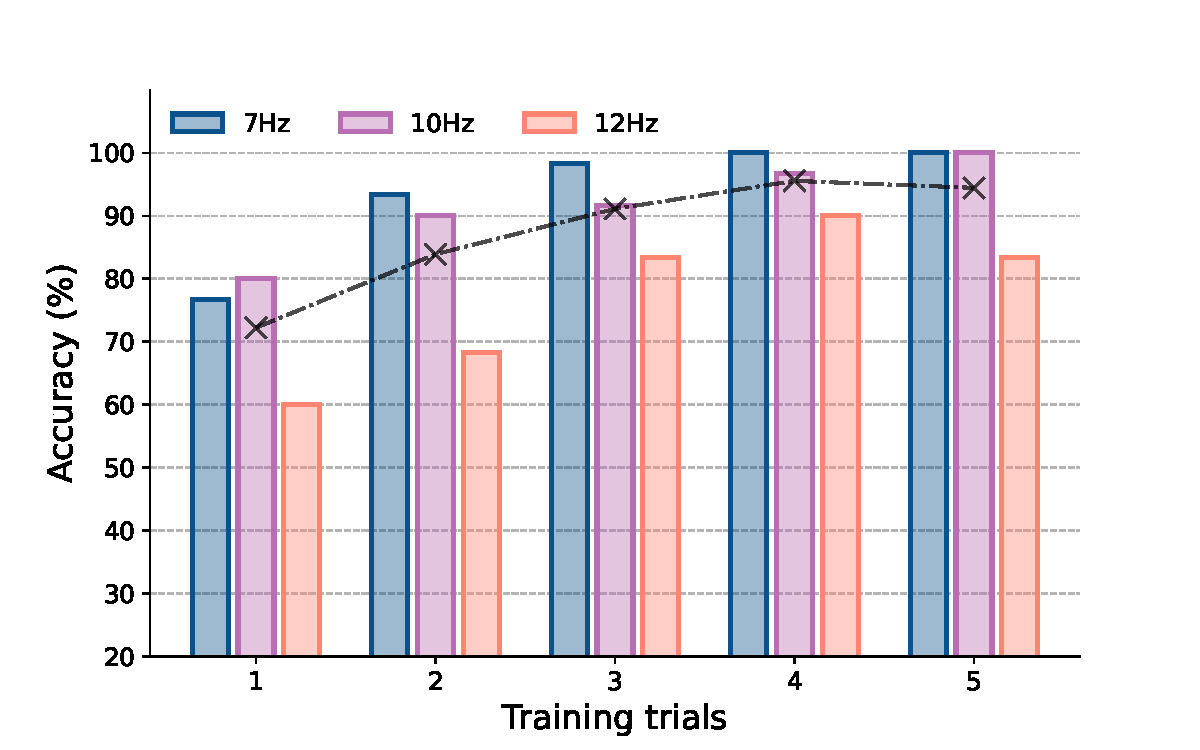
\includegraphics[clip,width=0.49\columnwidth]{report/C6 Results/assets/acc_Nt_gcca_Ns128.pdf}%
    \label{subfig:gcca-nt-ns128}
}
\hfill
\subfloat[$T = 4$s ($N_s=1024, N_s'=256$)]{%
    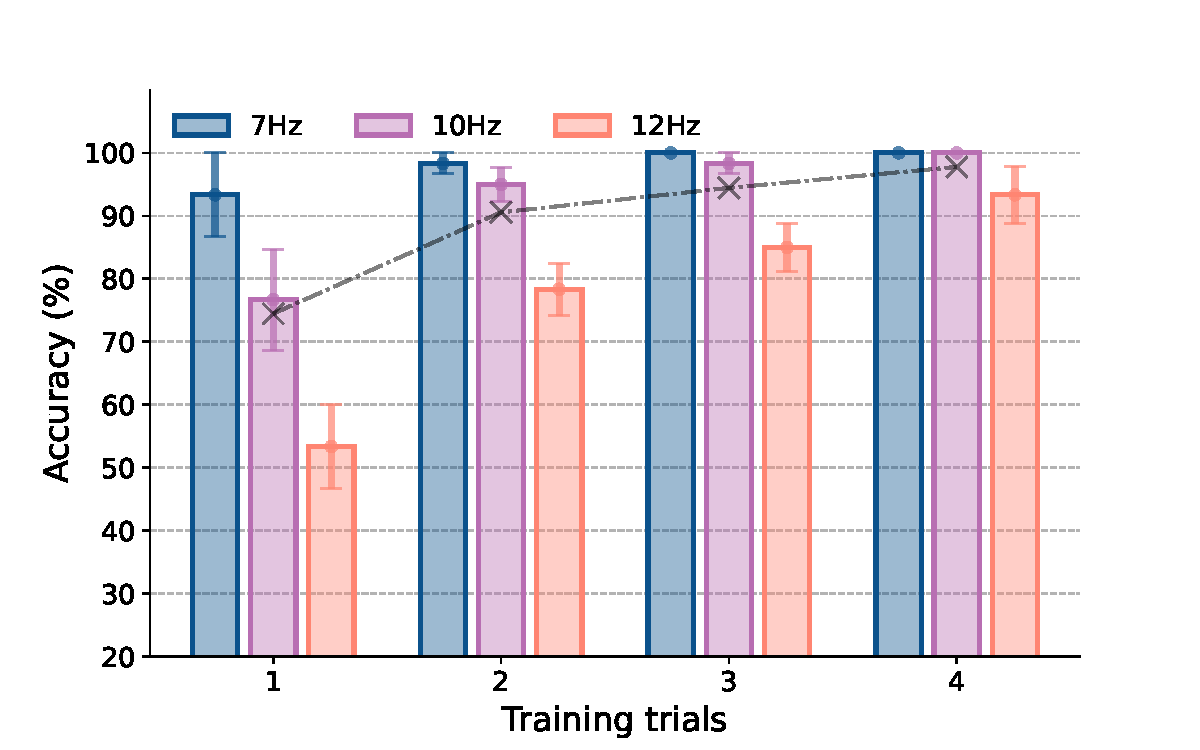
\includegraphics[clip,width=0.49\columnwidth]{report/C6 Results/assets/acc_Nt_gcca_Ns256.pdf}%
    \label{subfig:gcca-nt-ns256}
}

\caption[GCCA decoding accuracy: effect of varying the number of training (calibration) trials $N_t$ on validation accuracy for recording windows of varying length $T$.]{\textbf{GCCA decoding accuracy}: effect of varying the number of training (calibration) trials $N_t$ on validation accuracy for recording windows of varying length $T$. In each subfigure, all trials are of equal length $T$ seconds which equates to $N_s$ samples at $f_s=256$Hz and $N_s'$ samples at the downsampled rate of $f_s'=64$Hz. Crosses connected with dashed traces denote average decoding accuracy across stimulus frequencies for a given $N_t=n, \, n\in\{1, \dots, 5\}$.}
\label{fig:gcca-acc-nt}
\end{figure}


%% Experiments with varying Nt: MsetCCA
\begin{figure}[htp]
\subfloat[$T = 0.75$s ($N_s=192, N_s'=48$)]{%
    \label{subfig:gcca-nt-ns48}
    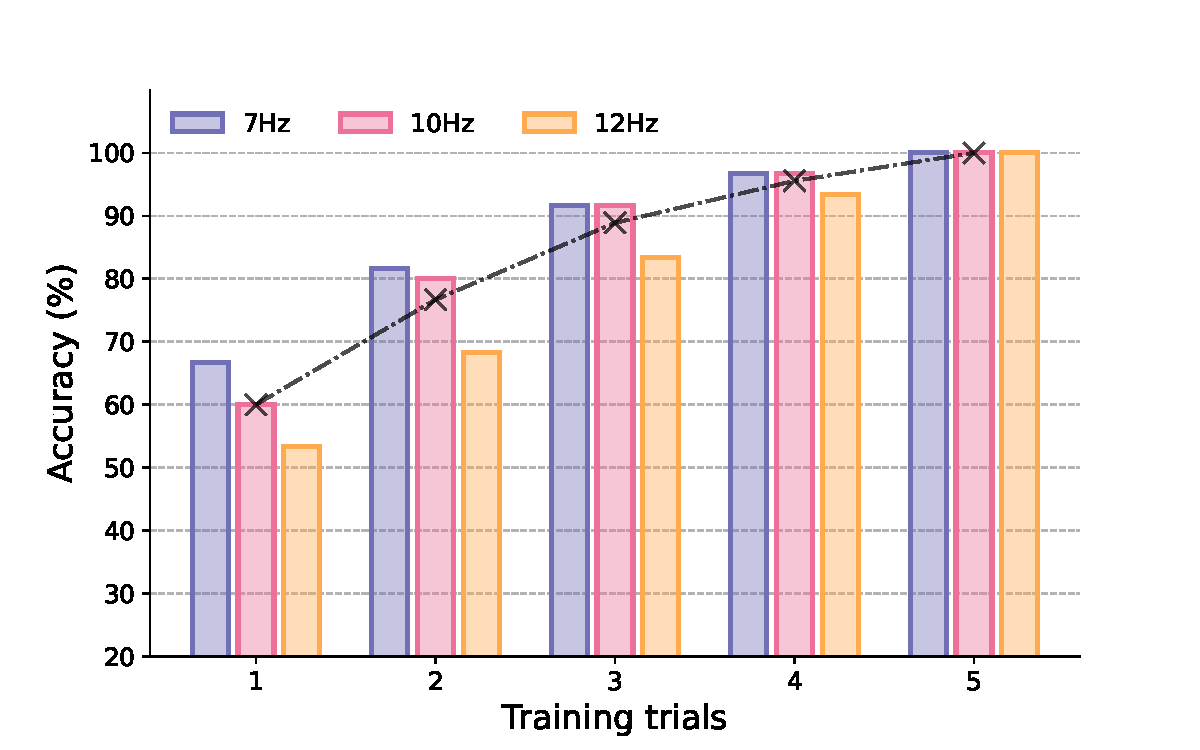
\includegraphics[clip,width=0.49\columnwidth]{report/C6 Results/assets/acc_Nt_mcca_Ns48.pdf}%
}
\hfill
\subfloat[$T = 1$s ($N_s=256, N_s'=64$)]{%
    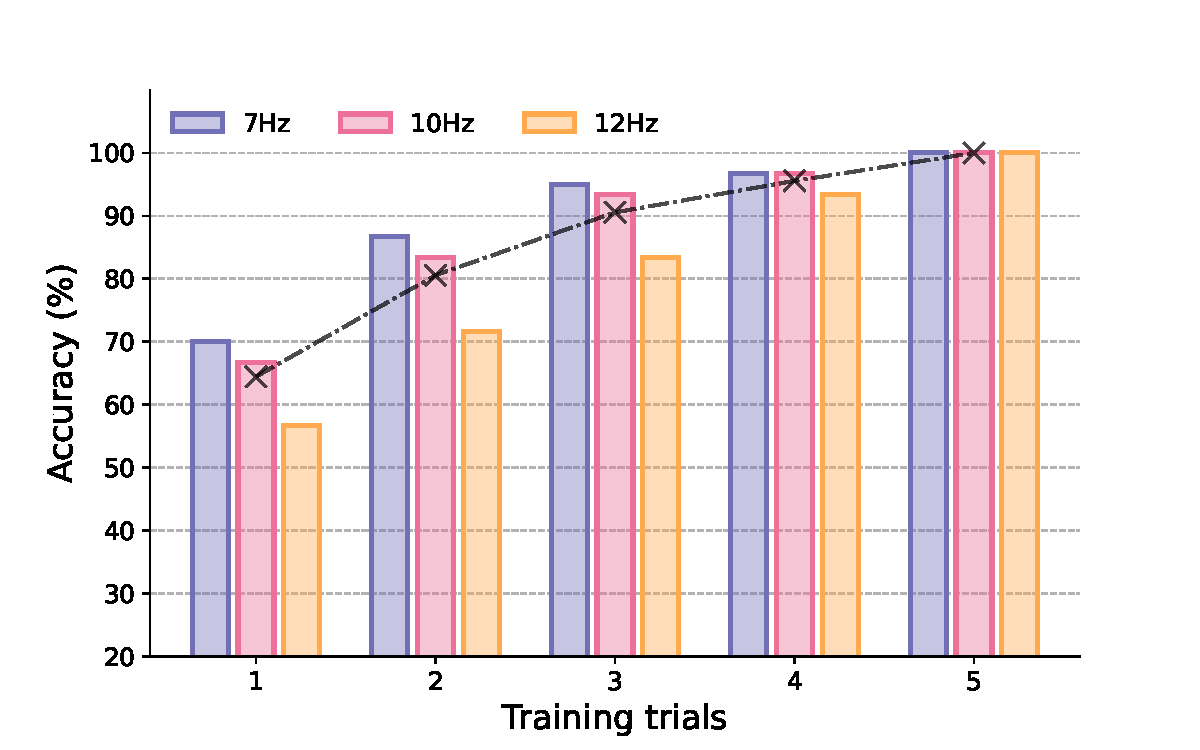
\includegraphics[clip,width=0.49\columnwidth]{report/C6 Results/assets/acc_Nt_mcca_Ns64.pdf}%
    \label{subfig:mset-nt-ns64}
}
% ensure there is a space below here!

\subfloat[$T = 2$s ($N_s=512, N_s'=128$)]{%
    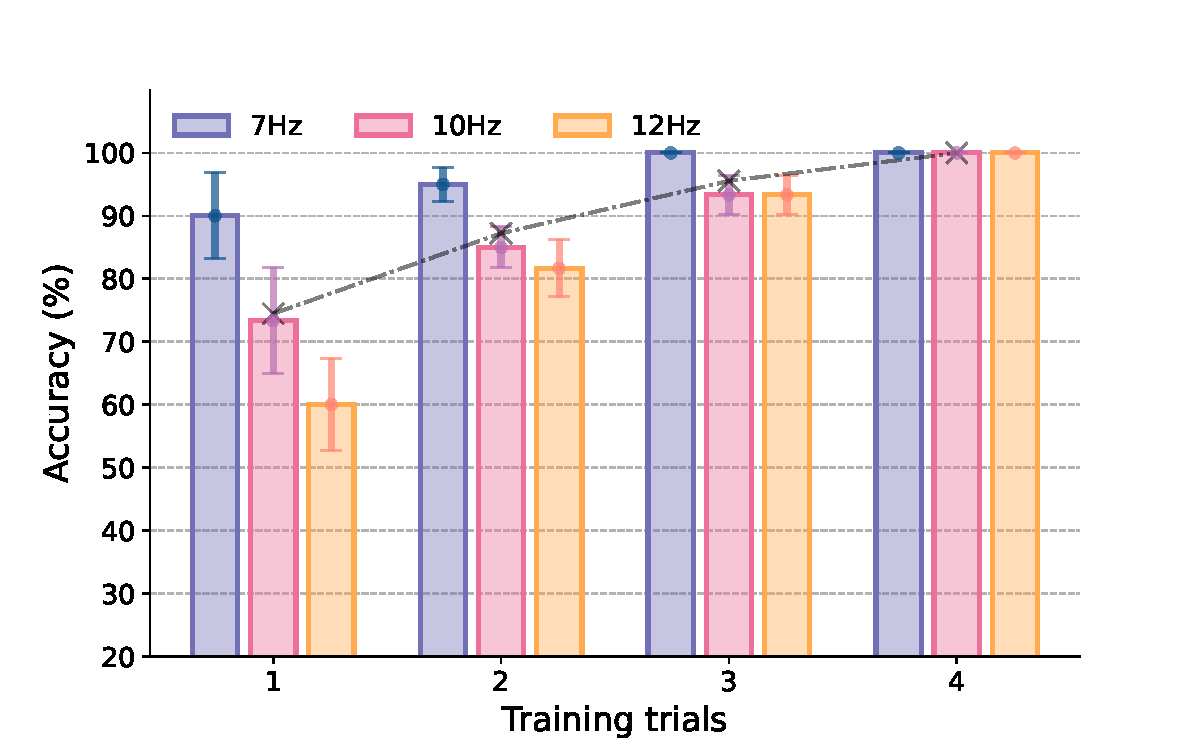
\includegraphics[clip,width=0.49\columnwidth]{report/C6 Results/assets/acc_Nt_mcca_Ns128.pdf}%
    \label{subfig:mset-nt-ns128}
}
\hfill
\subfloat[$T = 4$s ($N_s=1024, N_s'=256$)]{%
    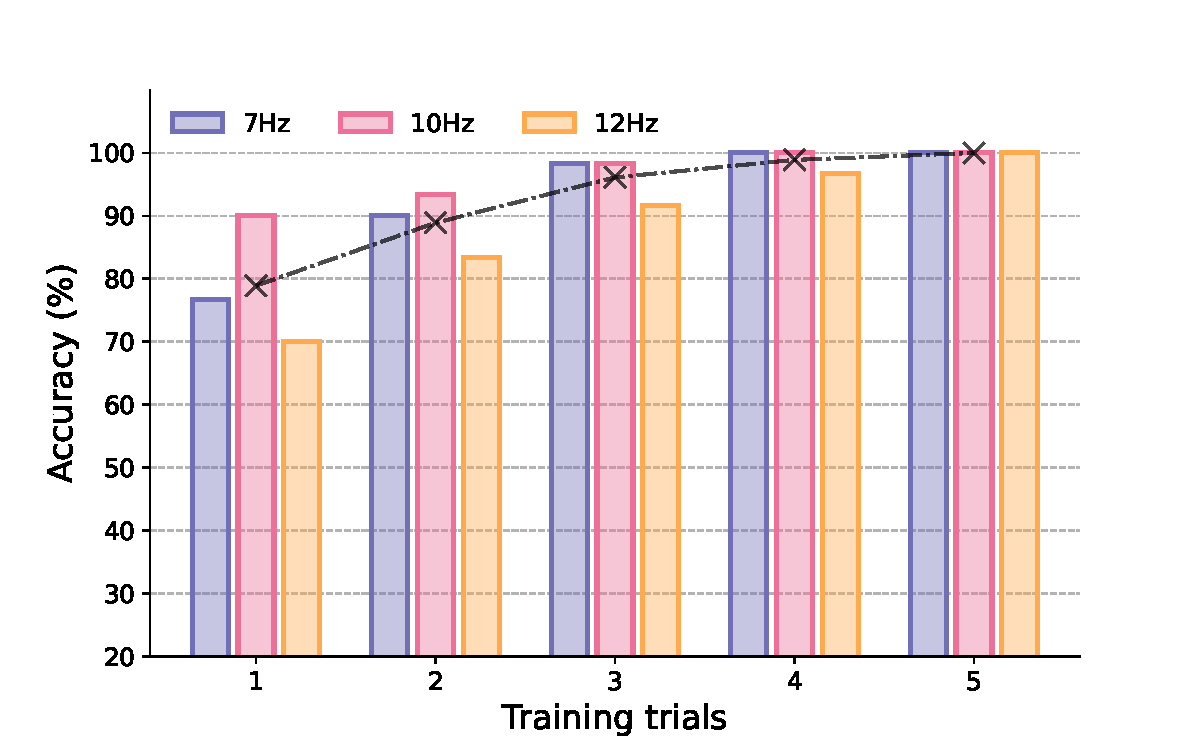
\includegraphics[clip,width=0.49\columnwidth]{report/C6 Results/assets/acc_Nt_mcca_Ns256.pdf}%
    \label{subfig:mset-nt-ns256}
}

\caption[MsetCCA decoding accuracy: effect of varying the number of training (calibration) trials $N_t$ on validation accuracy for recording windows of varying length $T$.]{\textbf{MsetCCA decoding accuracy}: effect of varying the number of training (calibration) trials $N_t$ on validation accuracy for recording windows of varying length $T$. In each subfigure, all trials are of equal length $T$ seconds which equates to $N_s$ samples at $f_s=256$Hz and $N_s'$ samples at the downsampled rate of $f_s'=64$Hz. Crosses connected with dashed traces denote average decoding accuracy across stimulus frequencies for a given $N_t=n, \, n\in\{1, \dots, 5\}$.}
\label{fig:mset-acc-nt}
\end{figure}

%% [SAMPLING LENGTH] Experiments with varying Ns: GCCA
\begin{figure}[htp]
\subfloat[$N_t=1$]{%
    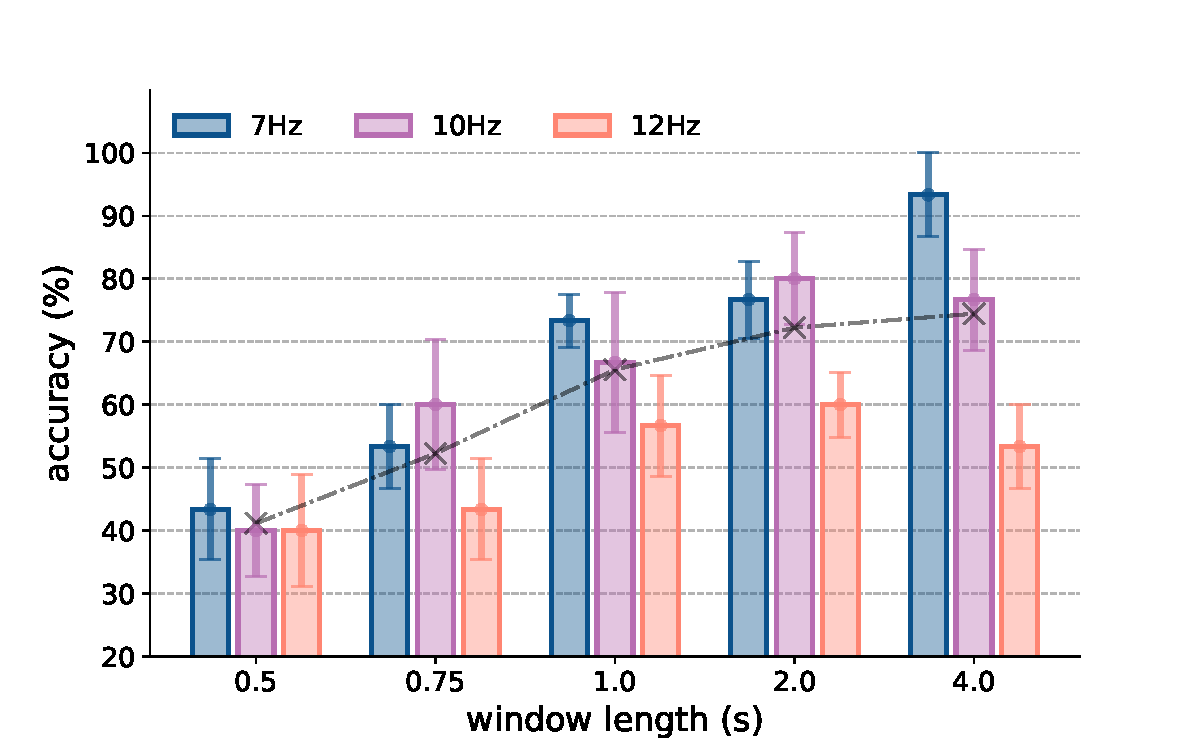
\includegraphics[clip,width=0.49\columnwidth]{report/C6 Results/assets/acc_Ns_gcca_Nt1.pdf}%
    \label{subfig:gcca-ns-nt1}
}
\hfill
\subfloat[$N_t=2$]{%
    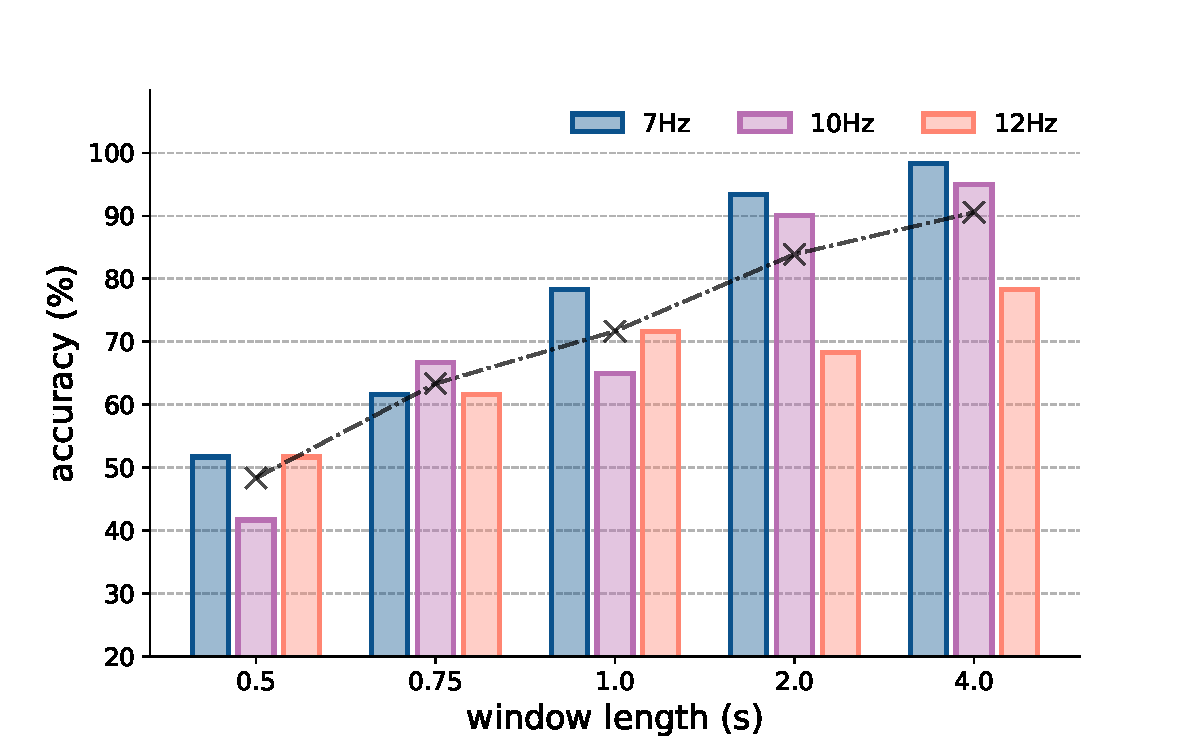
\includegraphics[clip,width=0.49\columnwidth]{report/C6 Results/assets/acc_Ns_gcca_Nt2.pdf}%
    \label{subfig:gcca-ns-nt2}
}
% ensure there is a space below here!

\subfloat[$N_t=3$)]{%
    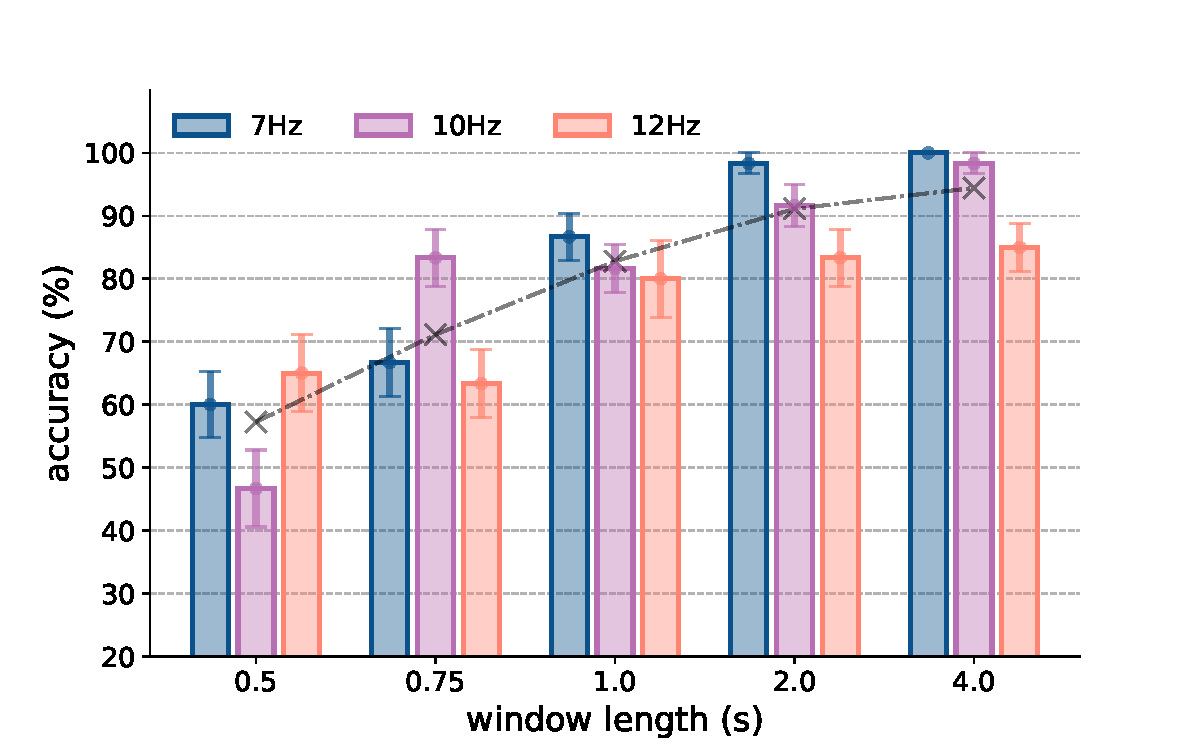
\includegraphics[clip,width=0.49\columnwidth]{report/C6 Results/assets/acc_Ns_gcca_Nt3.pdf}%
    \label{subfig:gcca-ns-nt3}
}
\hfill
\subfloat[$N_t=4$]{%
    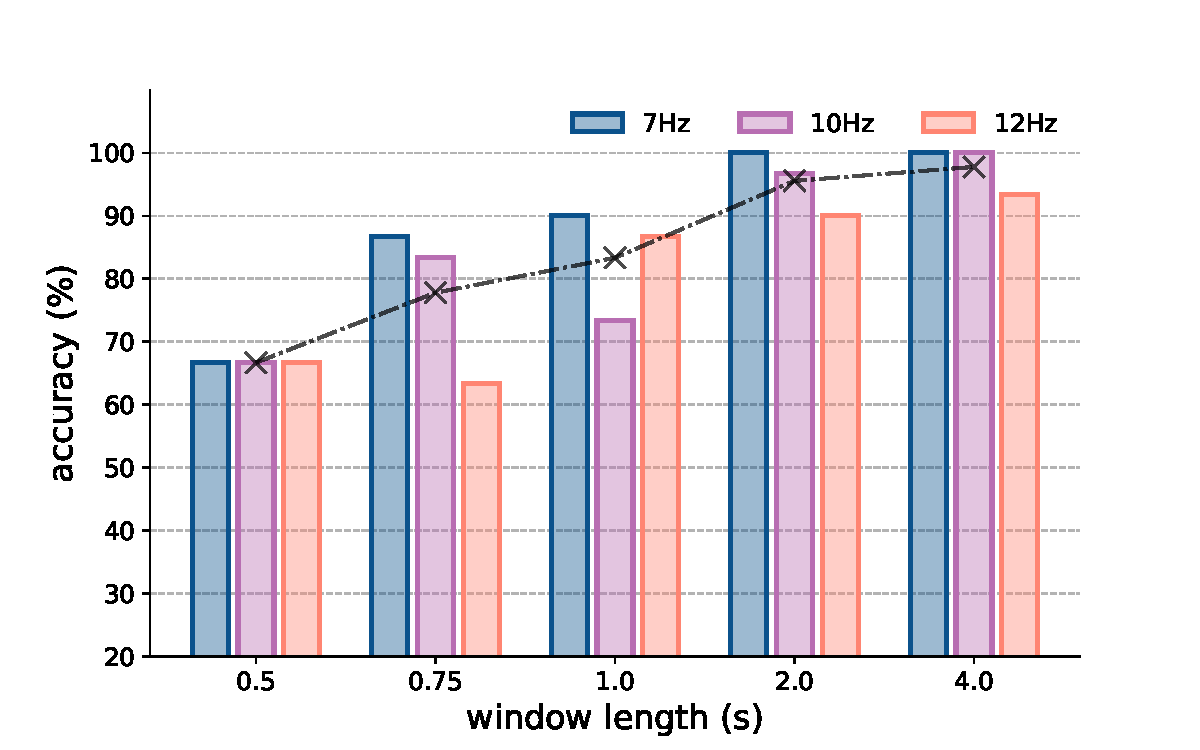
\includegraphics[clip,width=0.49\columnwidth]{report/C6 Results/assets/acc_Ns_gcca_Nt4.pdf}%
    \label{subfig:gcca-ns-nt4}
}

\caption[GCCA decoding accuracy: effect of varying recording window length $T$ on validation accuracy for different numbers of calibration trails $N_t$]{\textbf{GCCA decoding accuracy}: effect of varying recording window length $T$ on validation accuracy for different numbers of calibration trails $N_t$. In each subfigure, all results were computed using $N_t=n, \, n\in\{1, \dots, 4\}$ calibration trials. Crosses connected with dashed traces denote average decoding accuracy across stimulus frequencies for a given a given window length $T$.}
\label{fig:gcca-acc-ns}
\end{figure}

%% [SAMPLING LENGTH] Experiments with varying Ns: MsetCCA
\begin{figure}[htp]
\subfloat[$N_t=1$]{%
    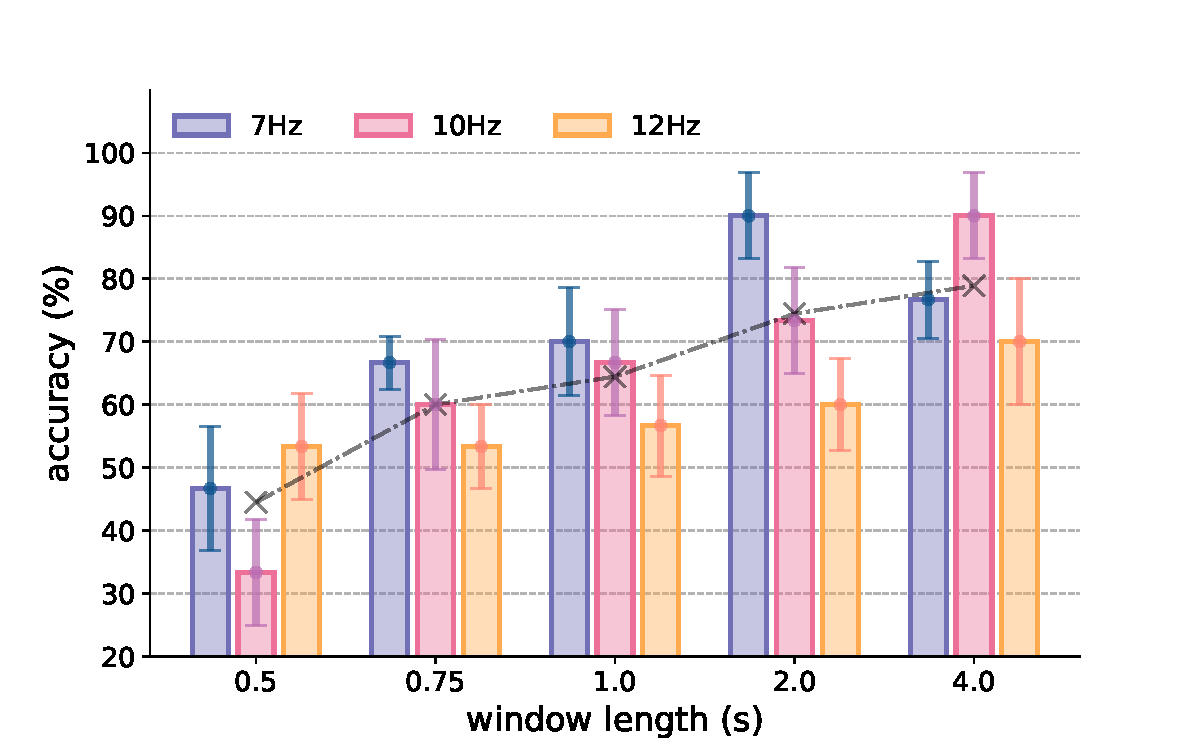
\includegraphics[clip,width=0.49\columnwidth]{report/C6 Results/assets/acc_Ns_mcca_Nt1.pdf}%
    \label{subfig:mcca-ns-nt1}
}
\hfill
\subfloat[$N_t=2$]{%
    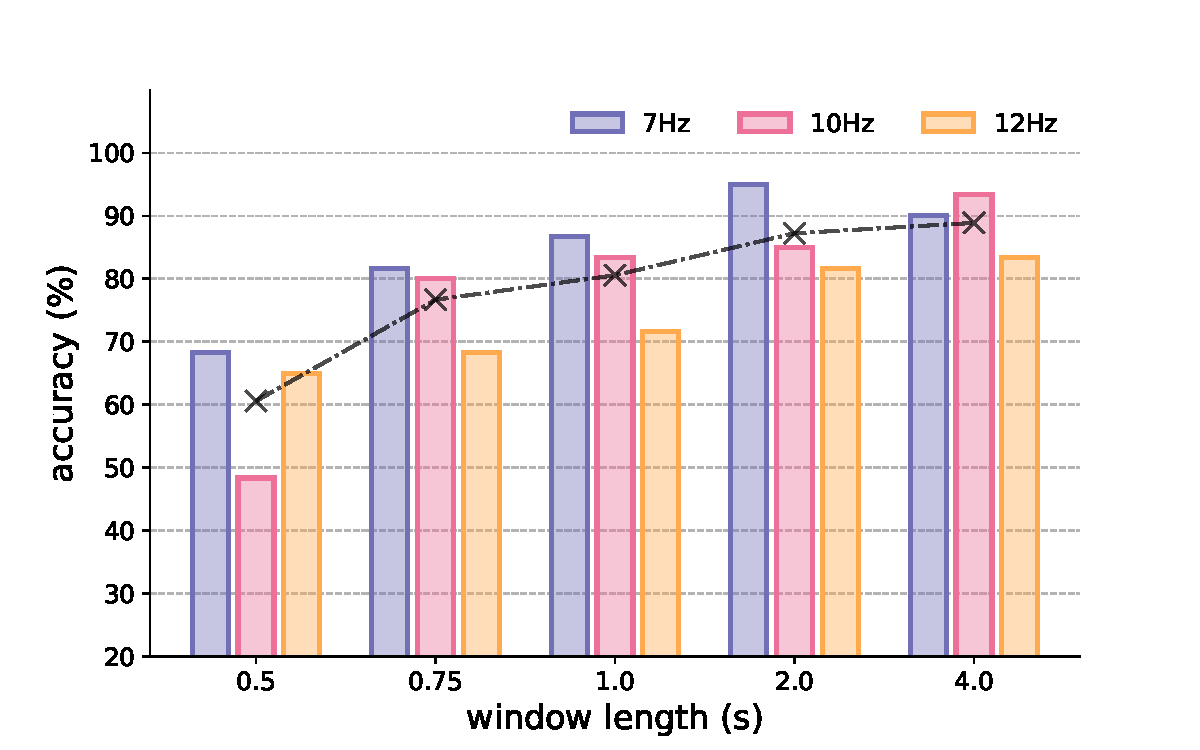
\includegraphics[clip,width=0.49\columnwidth]{report/C6 Results/assets/acc_Ns_mcca_Nt2.pdf}%
    \label{subfig:mcca-ns-nt2}
}
% ensure there is a space below here!

\subfloat[$N_t=3$)]{%
    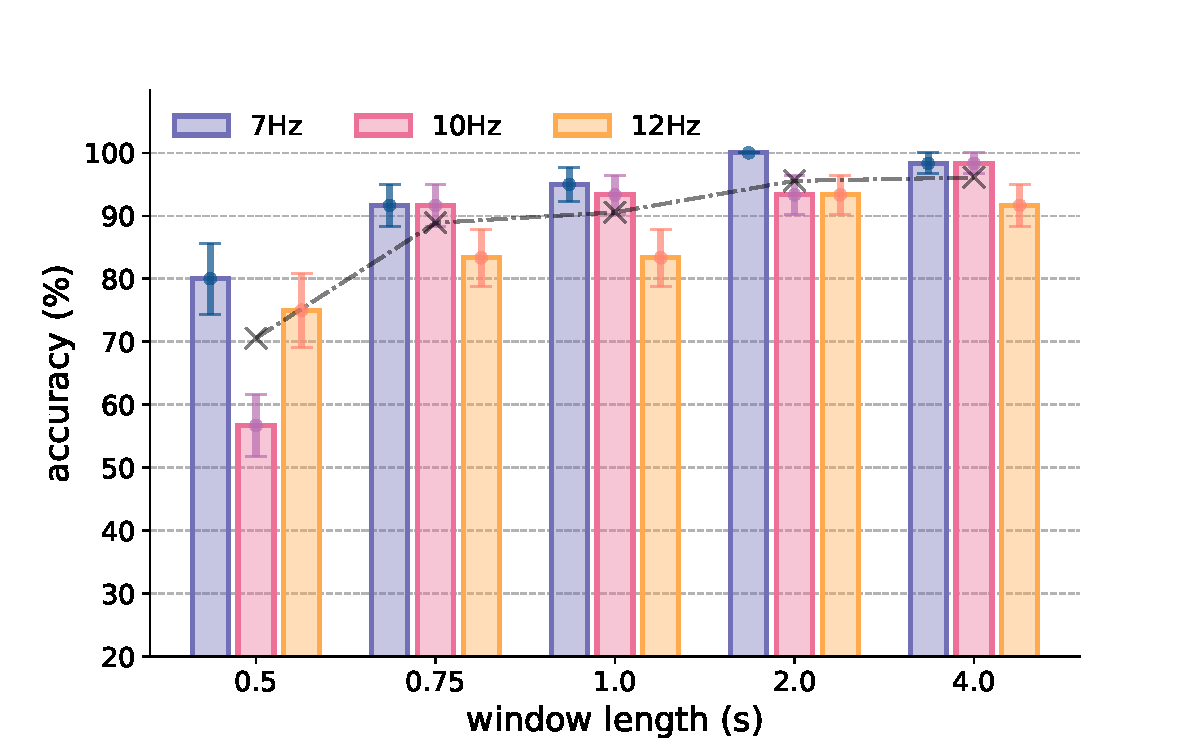
\includegraphics[clip,width=0.49\columnwidth]{report/C6 Results/assets/acc_Ns_mcca_Nt3.pdf}%
    \label{subfig:mcca-ns-nt3}
}
\hfill
\subfloat[$N_t=4$]{%
    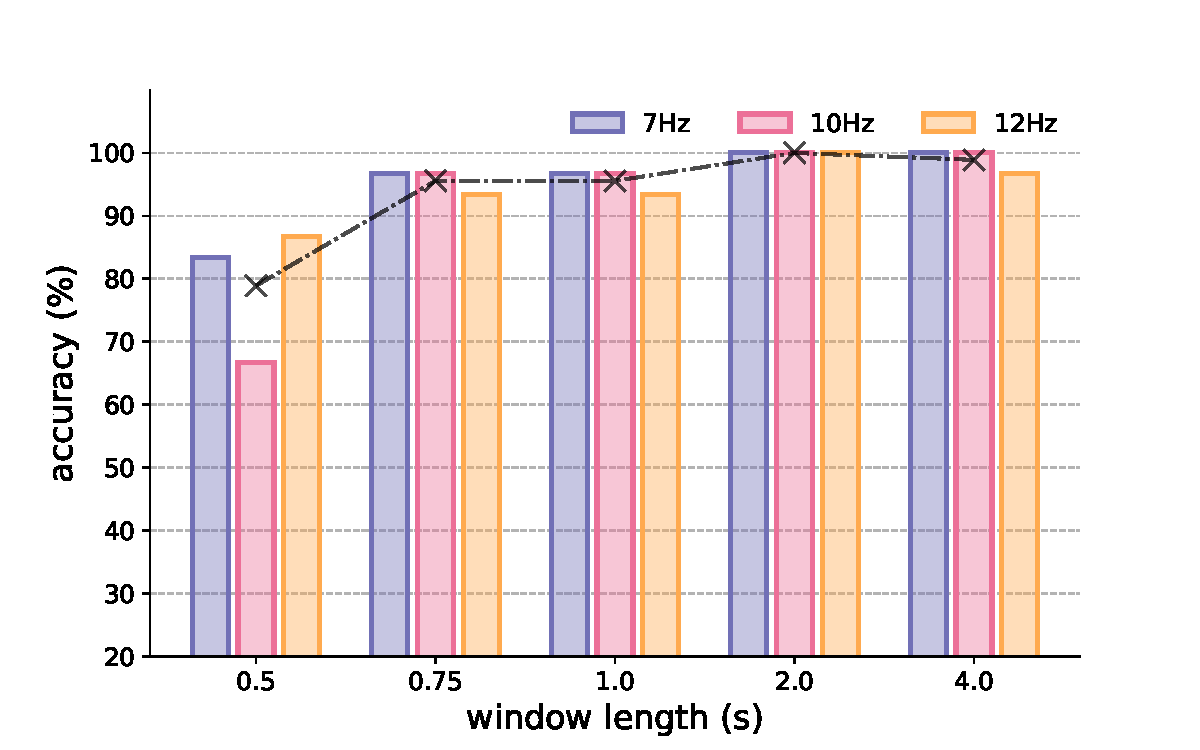
\includegraphics[clip,width=0.49\columnwidth]{report/C6 Results/assets/acc_Ns_mcca_Nt4.pdf}%
    \label{subfig:mcca-ns-nt4}
}

\caption[MsetCCA decoding accuracy: effect of varying recording window length $T$ on validation accuracy for different numbers of calibration trails $N_t$]{\textbf{MsetCCA decoding accuracy}: effect of varying recording window length $T$ on validation accuracy for different numbers of calibration trails $N_t$. In each subfigure, all results were computed using $N_t=n, \, n\in\{1, \dots, 4\}$ calibration trials. Crosses connected with dashed traces denote average decoding accuracy across stimulus frequencies for a given a given window length $T$.}
\label{fig:mcca-acc-ns}
\end{figure}

% \begin{figure}
%      \centering
%      \begin{subfigure}[b]{0.3\textwidth}
%          \centering
%          \includegraphics[width=\textwidth]{acc}
%          \caption{$y=x$}
%          \label{fig:y equals x}
%      \end{subfigure}
%      \hfill
%      \begin{subfigure}[b]{0.3\textwidth}
%          \centering
%          \includegraphics[width=\textwidth]{graph2}
%          \caption{$y=3sinx$}
%          \label{fig:three sin x}
%      \end{subfigure}
%      \hfill
%      \begin{subfigure}[b]{0.3\textwidth}
%          \centering
%          \includegraphics[width=\textwidth]{graph3}
%          \caption{$y=5/x$}
%          \label{fig:five over x}
%      \end{subfigure}
%         \caption{Three simple graphs}
%         \label{fig:three graphs}
% \end{figure}

% \section{Experiments using Benchmark Data}
